\chapter{Results}
\label{chap:Results}

\section{Experimental Setup} \label{sec:expt-info}
All results presented in this chapter are generated on a supercomputing hardware cluster with a dual-socket 64-core AMD EPYC 7763 (``Milan") CPU and NVIDIA A100 40GB HBM2 GPU.
The system has 256 GB of DDR4 memory with 1.5 TB swap memory via high-performance-SSD.
The program is compiled with NVCC (CUDA 11.7, driver version 515.48) SM version 80, and GCC 11.2 with the -O3 flag.
For a fair comparison, the baseline is also run on the same hardware platform with equivalent compilation flags.

The data graphs used for experiments are obtained from the Stanford Network Analysis Project (SNAP) \cite{snap}.
Table \ref{tab:graphs} summarizes the properties of these data graphs.

\begin{table}[tbp]
    \centering
    \caption{Data Graphs used for experiments}
    % \resizebox{\textwidth}{!}{%
    \begin{tabular}{@{}crrr@{}}
        \hline
        \multicolumn{1}{c}{\textbf{Graph}} & \multicolumn{1}{c}{$|\textbf{V}|$} & \multicolumn{1}{c}{$|\textbf{E}|$} & \multicolumn{1}{c}{\textbf{Max Degree}} \\ \hline
        as-skitter                         & 1,696,415                          & 11,095,298                         & 35,455                                  \\
        soc-pokec                          & 1,632,804                          & 22,301,964                         & 14,854                                  \\
        % com-dblp                           & 317,080                            & 1,049,866                          & 343                                     \\
        cit-patents                        & 3,774,768                          & 16,518,948                         & 793                                     \\
        % com-lj                             & 3,997,962                          & 34,681,189                         & 14,815                                  \\
        com-orkut                          & 3,072,441                          & 117,185,083                        & 33,313                                  \\
        % com-friendster                     & 65,608,366                         & 1,806,067,135                      & 5,214                                   \\
        com-youtube                        & 1,134,891                          & 5,975,248                          & 28,754                                  \\
        \hline
    \end{tabular}%
    % }
    \label{tab:graphs}
\end{table}

We use the common query graphs with central nodes that are generally used in subgraph enumeration literature.
Figure \ref{fig:queries} shows the query graphs used for experiments, these queries are adapted from \cite{PARSEC_VD}.
\textit{Clique} is a fully connected graph.
As a notation in Figures and Tables, we use cqx for \textit{clique} of size x and cqxm1 for size x \textit{clique} with one edge missing. Note, removing exactly one edge from a \textit{clique} gives a unique query due to symmetry.
\begin{figure}[t]
    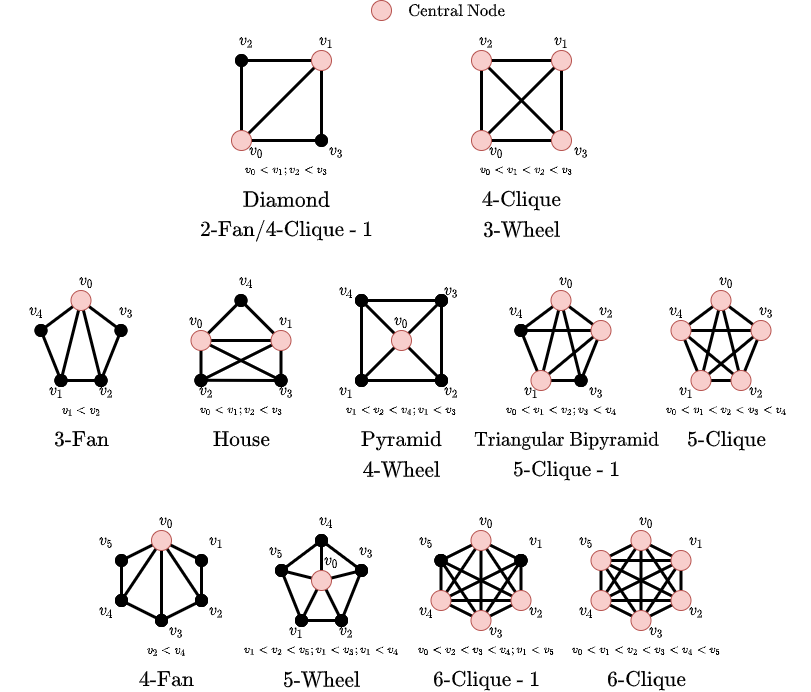
\includegraphics[width=\textwidth]{fig/improvements/Templates.png}
    \source{PARSEC \cite{PARSEC_VD}}
    \caption{Query Graphs used for experiments}
    \label{fig:queries}
\end{figure}

\section{Performance Criteria}
The performance is evaluated in terms of total processing time which includes query preprocessing, data graph preprocessing, and search tree traversal times.
We use the following rules for reporting run times:\
\begin{enumerate}
    \item For instances with total run times less than 1 second, the program is executed 5 times and average times are reported.
    \item Time taken for compilation, reading data graphs, and printing all enumerations is not considered for the baseline and our implementation.
    \item The baseline presents two parallelization schemes with the comment that the edge per block scheme works better than node per block for templates of size greater than five. This observation is used for fixing one parallelization scheme for comparison.
    \item Instances that take more than 12,000 seconds ($\sim 3.3$ hours) are terminated, and their times are not reported. The corresponding speedup values are reported as blank in all tables.
\end{enumerate}


\section{Final Results and Analysis}



\begin{table}[h]
    \centering
    \caption{Speedups across all queries and data graphs}
    \resizebox{\textwidth}{!}{%
        \begin{tabular}{c|ccccc|c}
            \textbf{Queries}  & \textbf{soc-pokec} & \textbf{com-youtube} & \textbf{cit-patents} & \textbf{com-orkut} & \textbf{as-skitter} & \textbf{Geo Mean} \\
            \hline
            Tri               & 1.49               & 2.11                 & 1.00                 & 0.73               & 1.95                & 1.35              \\
            Diamond           & 1.44               & 2.31                 & 1.00                 & 0.92               & 2.08                & 1.45              \\
            cq4               & 1.47               & 2.51                 & 1.03                 & 0.76               & 1.85                & 1.40              \\
            cq5m1             & 1.41               & 2.62                 & 1.08                 & 1.23               & 1.76                & 1.54              \\
            cq5               & 1.46               & 3.04                 & 1.07                 & 1.13               & 1.83                & 1.58              \\
            house             & 1.41               & 2.27                 & 1.08                 & 1.36               & 3.45                & 1.75              \\
            pyramid           & 1.50               & 14.65                & 1.15                 & 4.5                & 9.75                & 4.06              \\
            fan3              & 1.50               & 9.38                 & 1.26                 & 3.59               & 5.89                & 3.27              \\
            cq6m1             & 4.19               & 3.09                 & 5.47                 & 2.41               & 1.44                & 3.01              \\
            fan4              & 3.41               & 5.82                 & 2.62                 & --                 & --                  & 3.73              \\
            wheel5            & 3.39               & 5.93                 & 2.10                 & --                 & --                  & 3.48              \\
            cq6               & 5.68               & 3.65                 & 5.76                 & 4.48               & 2.01                & 4.04              \\
            cq7m1             & 3.19               & 3.14                 & 5.11                 & 1.47               & 1.11                & 2.42              \\
            cq7               & 4.43               & 3.96                 & 5.45                 & 2.01               & 1.32                & 3.03              \\
            cq8m1             & 2.32               & 2.88                 & 3.25                 & 1.32               & --                  & 2.31              \\
            cq8               & 3.55               & 4.06                 & 5.15                 & 1.58               & --                  & 3.29              \\
            cq9m1             & 1.44               & 2.93                 & 2.65                 & 1.32               & --                  & 1.96              \\
            cq9               & 2.32               & 4.06                 & 3.67                 & 1.52               & --                  & 2.69              \\
            \hline
            \textbf{Geo Mean} & 2.25               & 3.74                 & 2.20                 & 1.61               & 2.29                & 2.33
        \end{tabular}%
    }
    \label{tab:speedups}
\end{table}

\begin{figure}
    \centering
    \subfigure[Data Graph: soc-pokec]{
        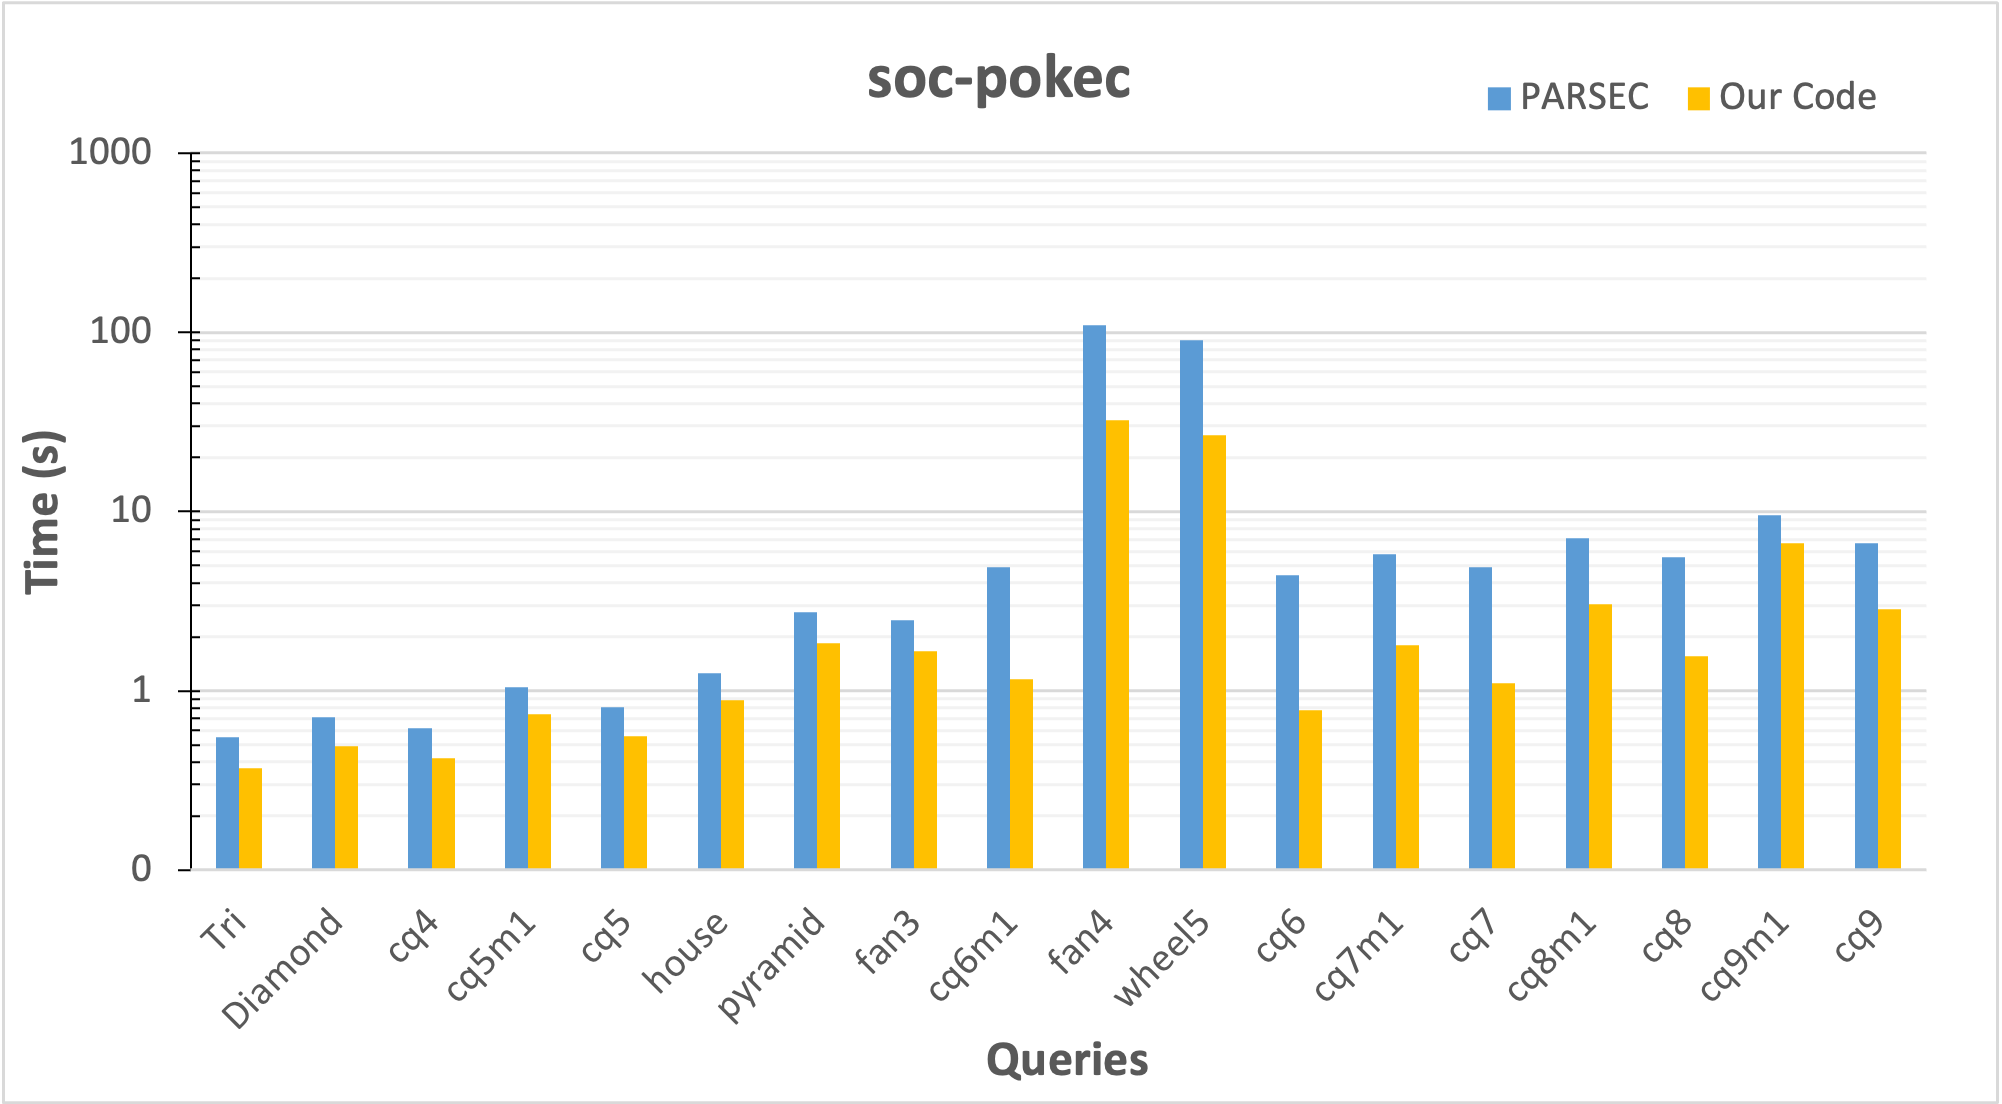
\includegraphics[width=\linewidth]{fig/Results/soc-pokec_times.png}
    }
    \subfigure[Data Graph: com-youtube]{
        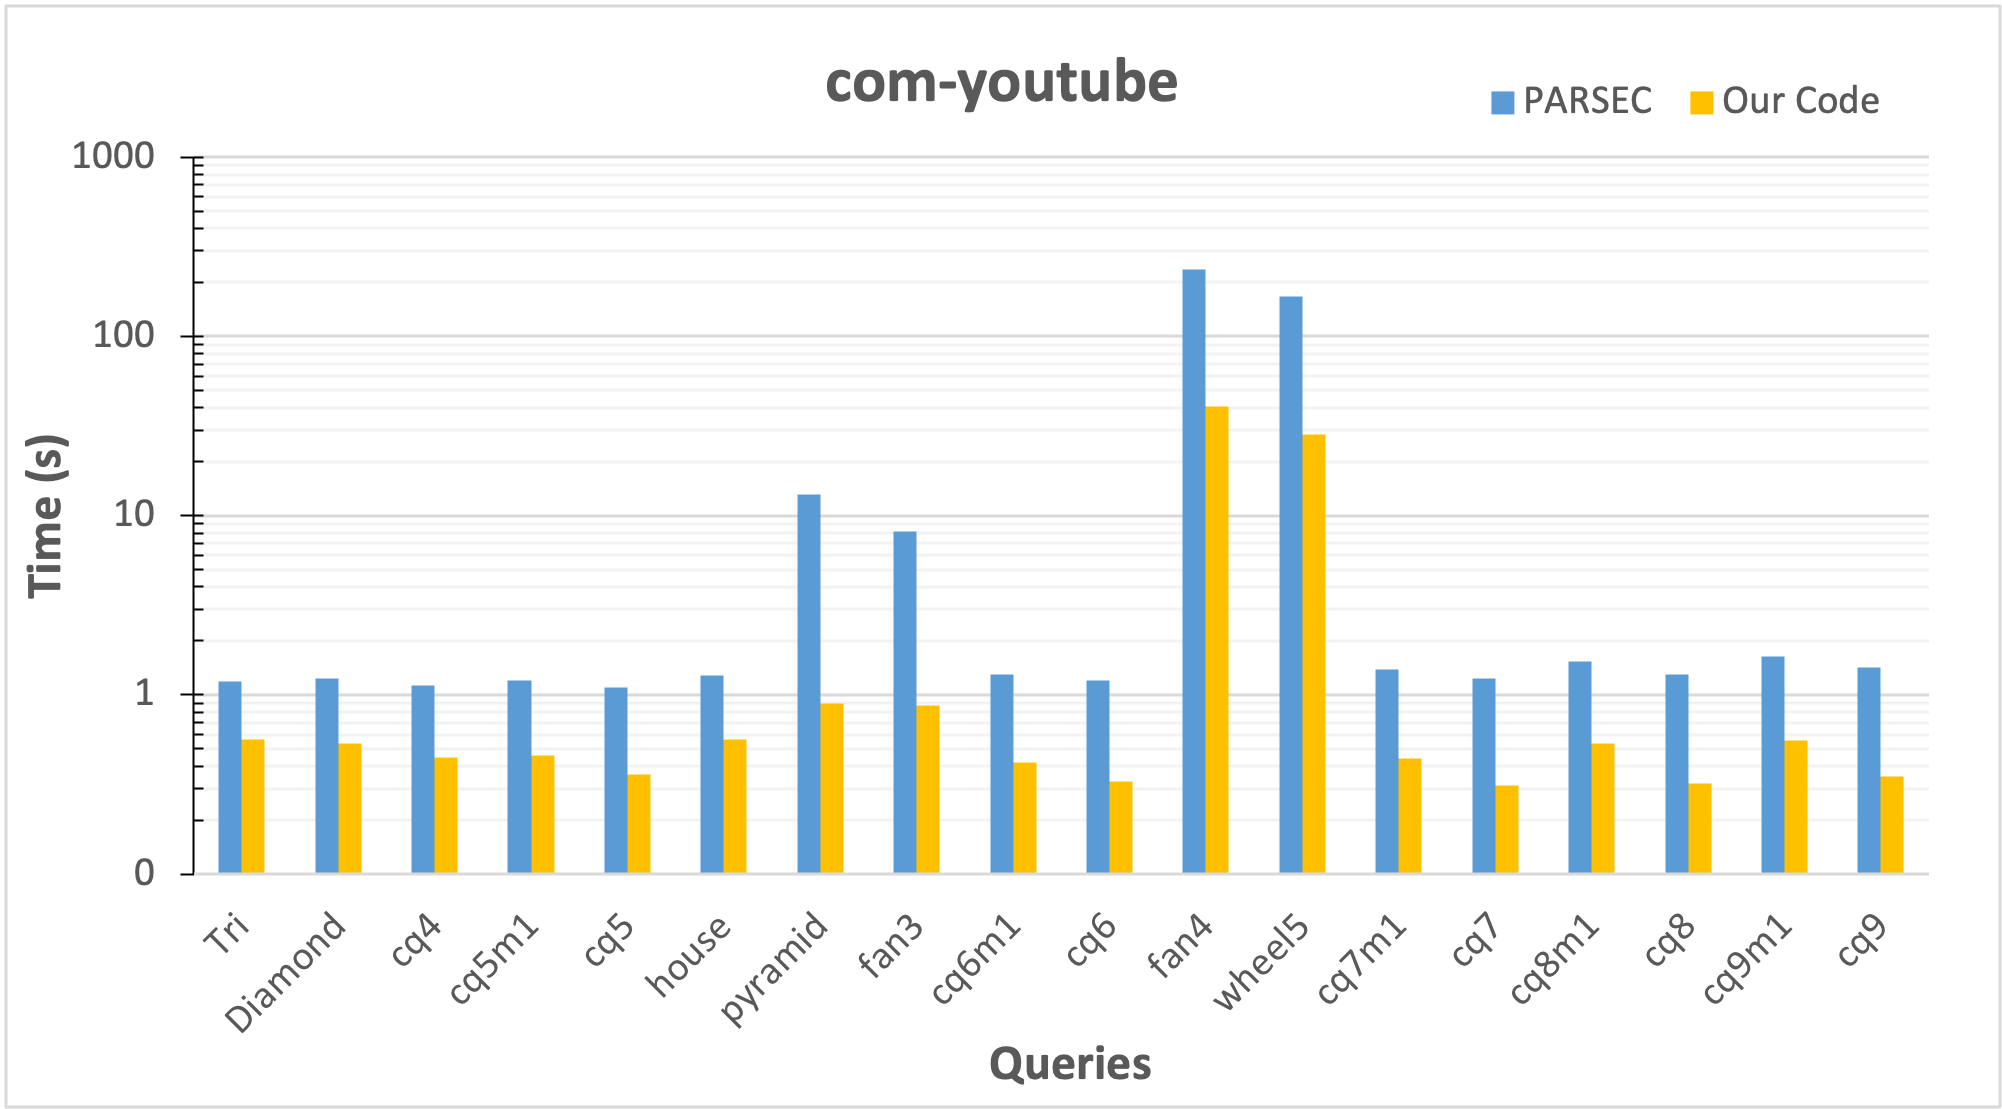
\includegraphics[width=\linewidth]{fig/Results/com-youtube_times.png}
    }
    \caption{Execution times and speedups compared to PARSEC \cite{PARSEC_VD}}
    \label{fig:gpu_comp}
\end{figure}
\begin{figure}\ContinuedFloat
    \centering
    \setcounter{subfigure}{2}
    \subfigure[Data Graph: cit-patents]{
        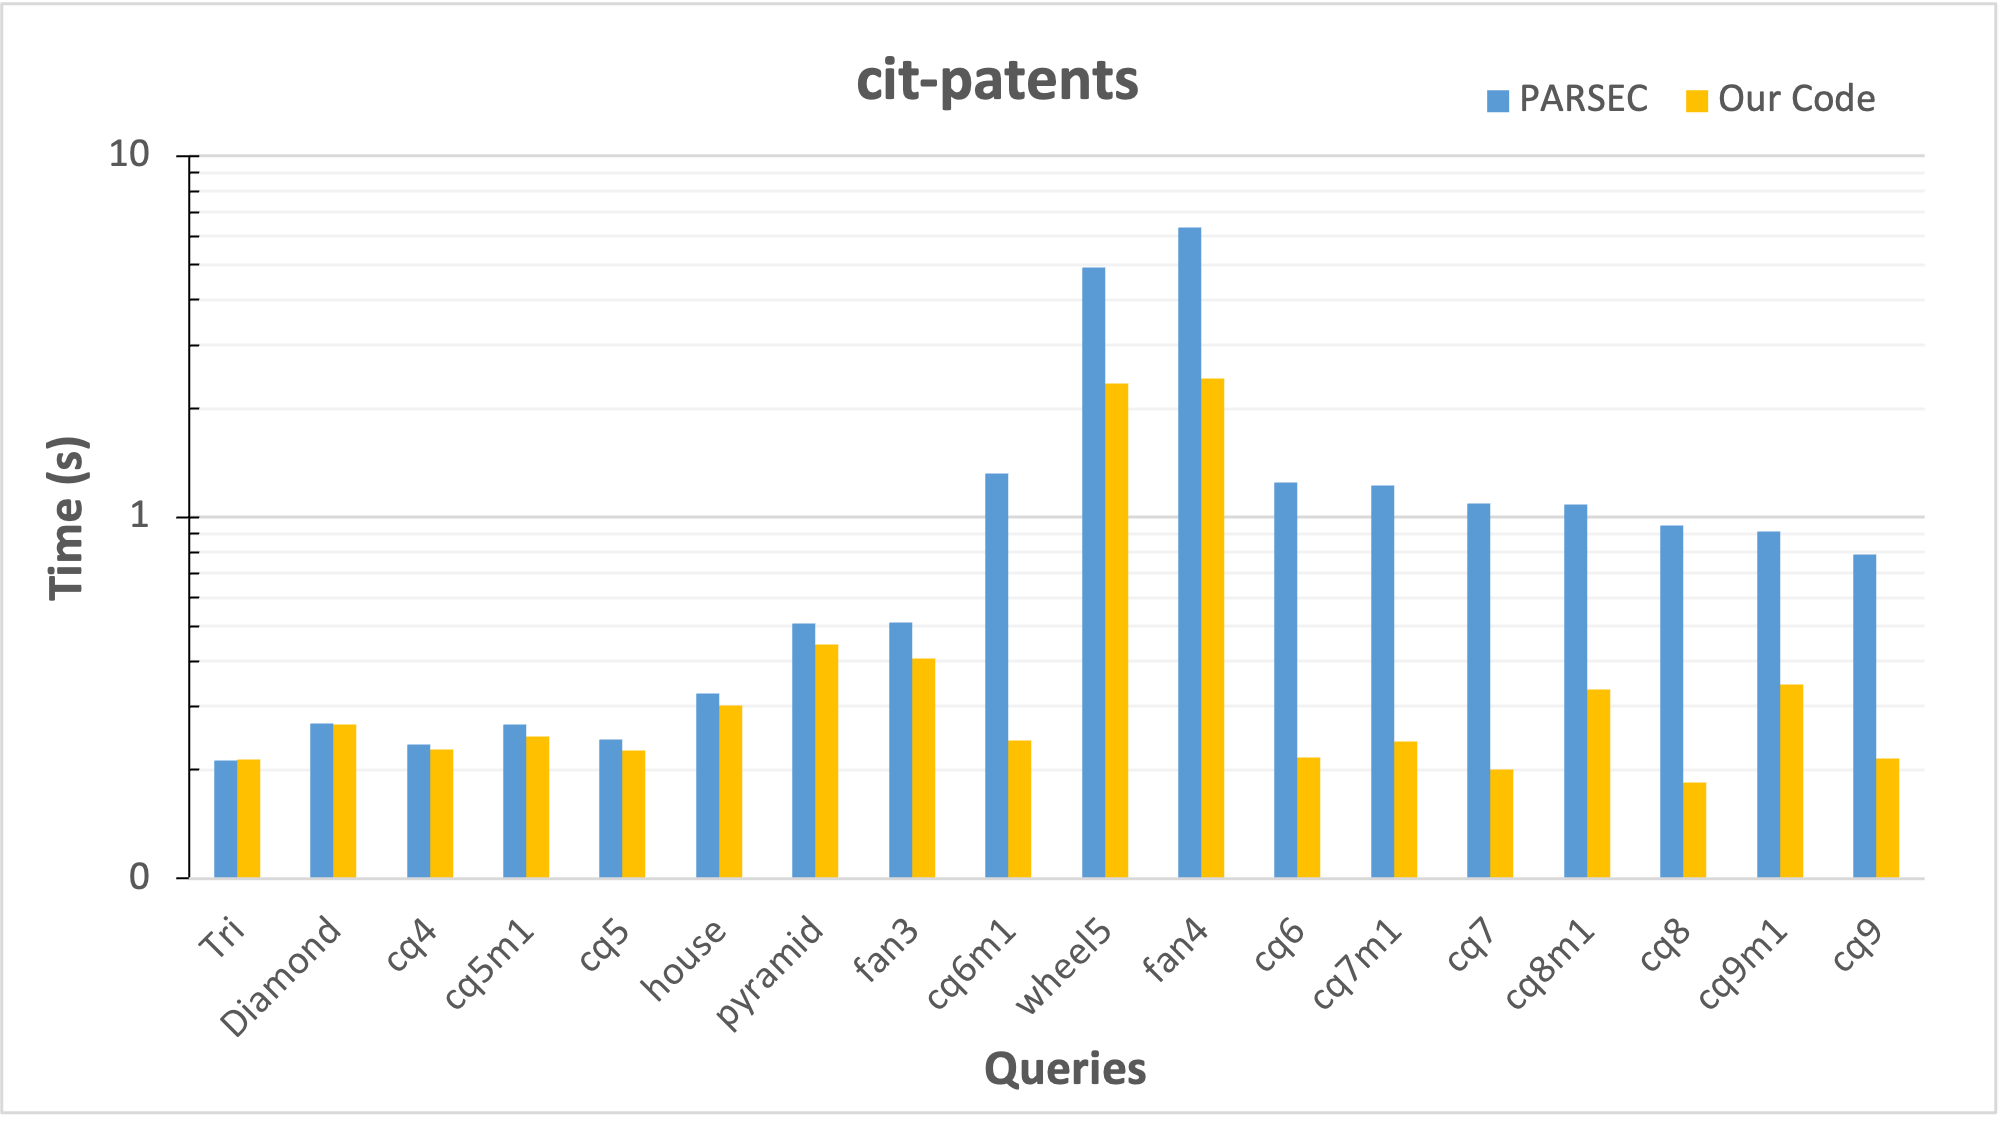
\includegraphics[width=\linewidth]{fig/Results/cit-patents_times.png}
    }
    \subfigure[Data Graph: com-orkut]{
        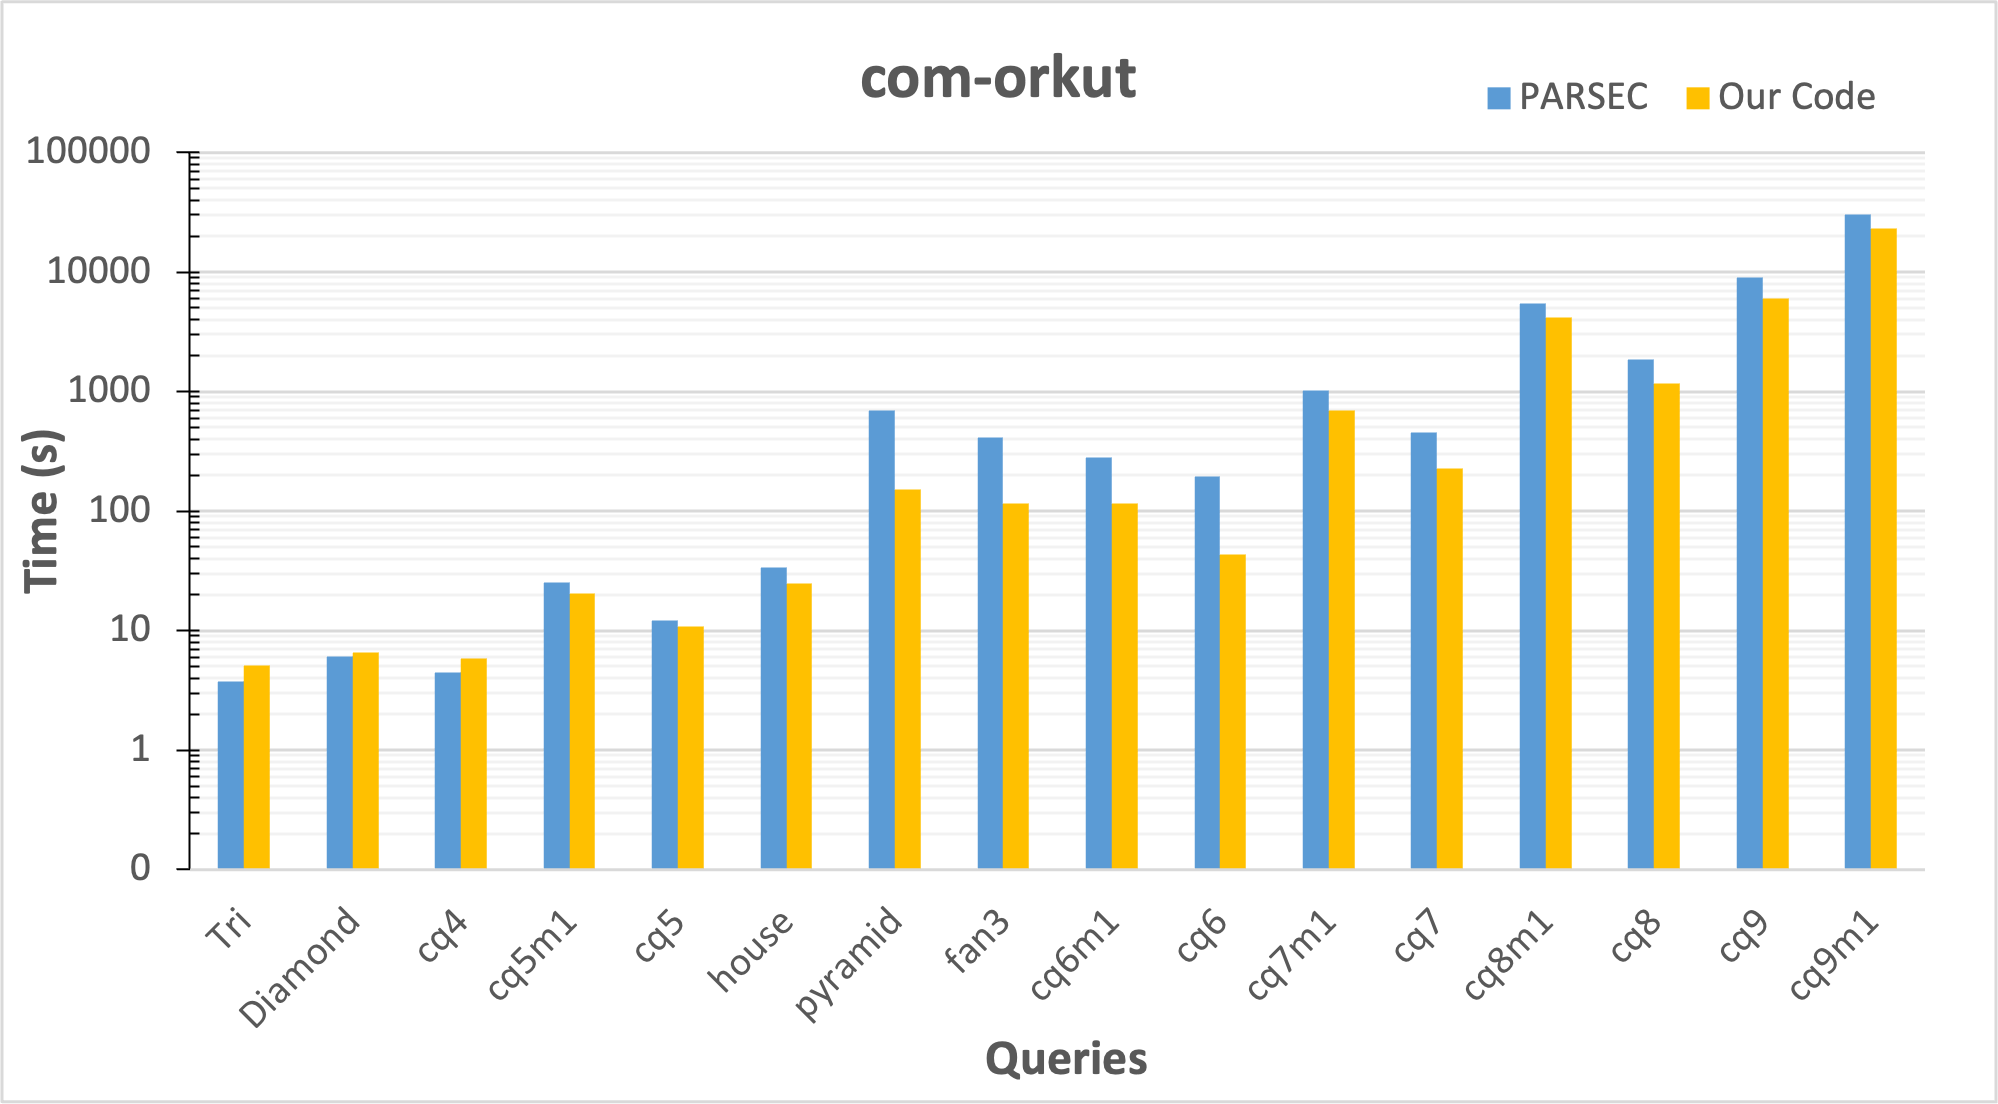
\includegraphics[width=\linewidth]{fig/Results/com-orkut_times.png}
    }
    \caption{Execution times and speedups compared to PARSEC \cite{PARSEC_VD}}
\end{figure}
\begin{figure}\ContinuedFloat
    \centering
    \setcounter{subfigure}{4}
    \subfigure[Data Graph: as-skitter]{
        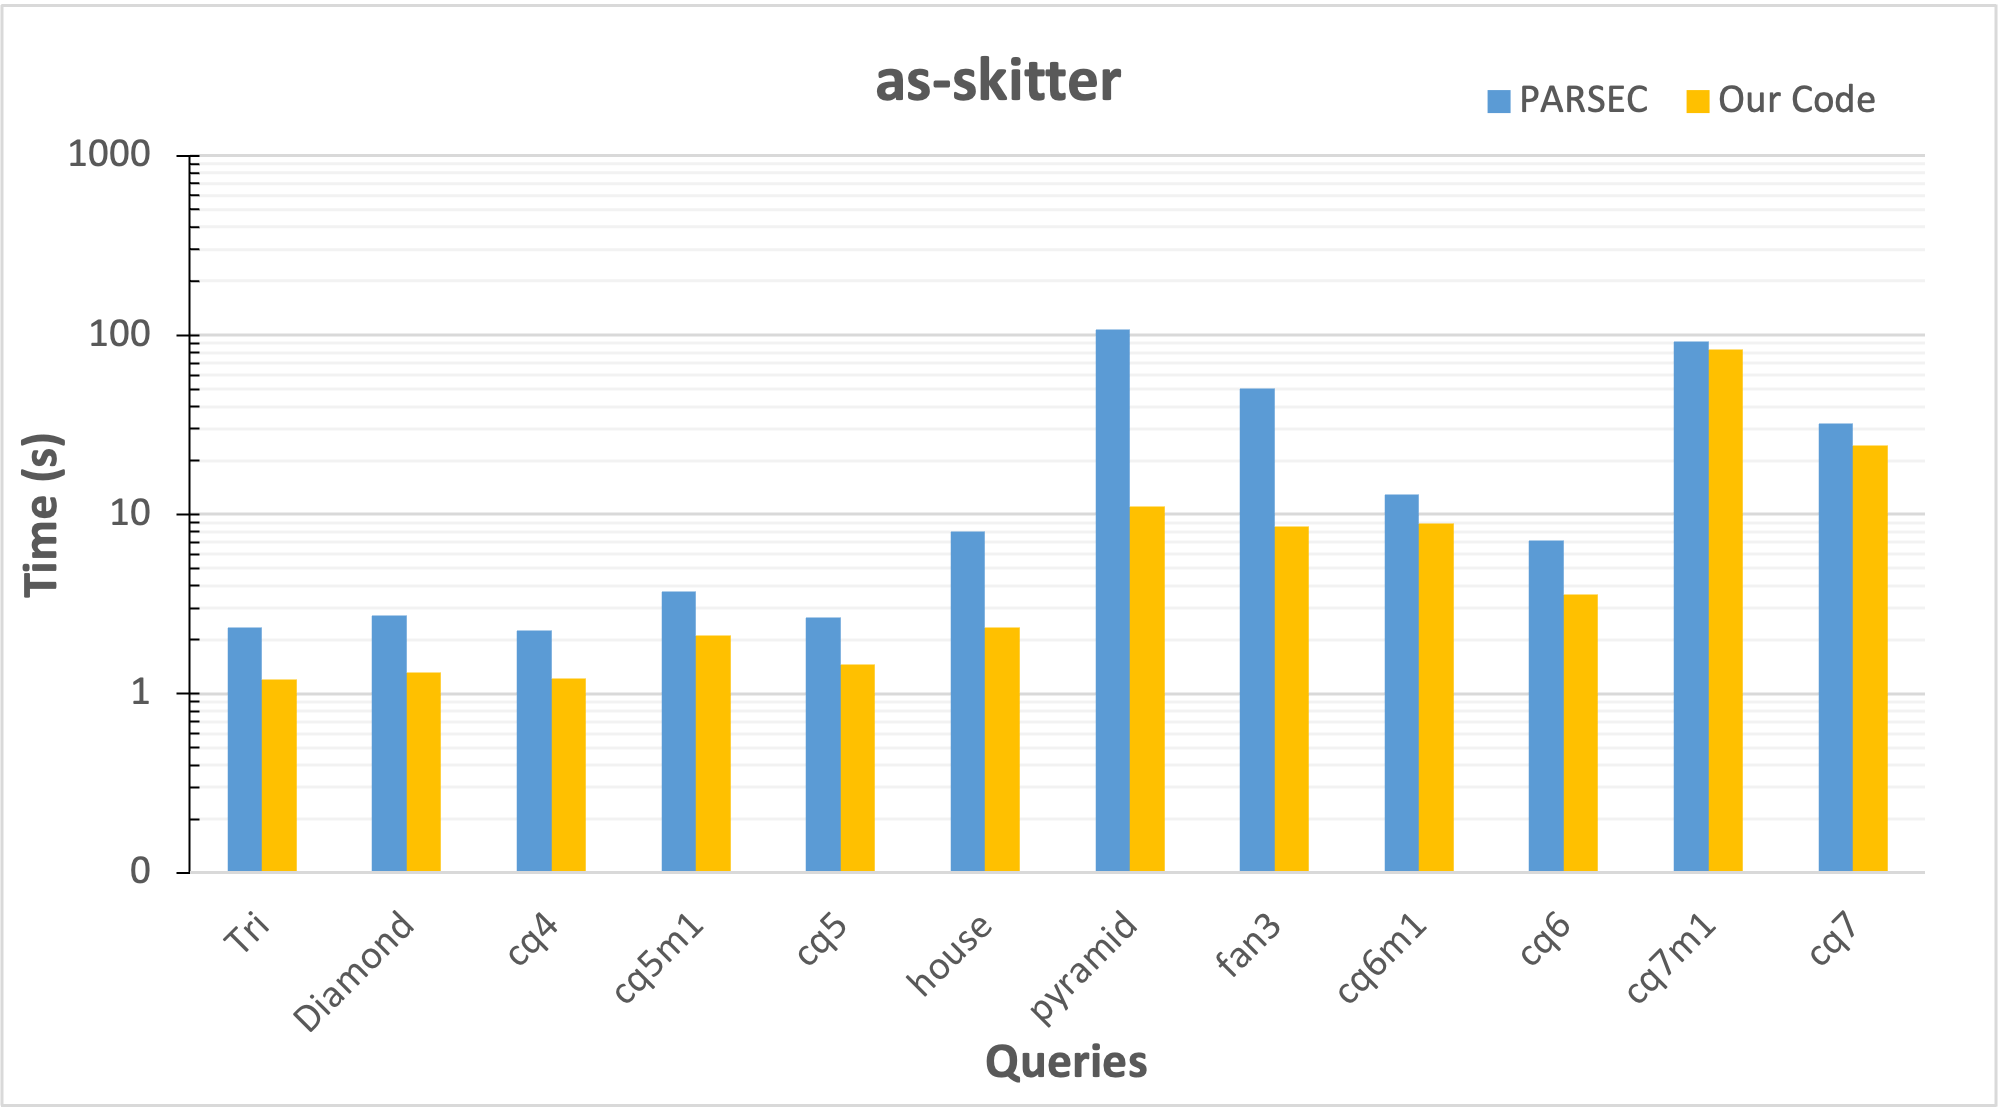
\includegraphics[width=\linewidth]{fig/Results/as-skitter_times.png}
    }
    \caption{Execution times and speedups compared to PARSEC \cite{PARSEC_VD}}
\end{figure}

% \begin{table}[]
%     \centering
%     \resizebox{\textwidth}{!}{%
%         \begin{tabular}{c|cccccccccccccccccc|c}\hline
%             \multirow{2}{*}{data graphs}                                                     & \multicolumn{18}{|c|}{} & \multirow{2}{*}{\textbf{\begin{tabular}[c]{@{}c@{}}Geo-mean\\ (across Queries)\end{tabular}}}                                                                                                                                                 \\
%                                                                                              & Tri                     & Diamond                                                                                       & cq4  & cq5m1 & cq5  & house & pyramid & fan3 & cq6m1 & fan4    & wheel5  & cq6  & cq7m1 & cq7  & cq8m1   & cq8     & cq9m1   & cq9     &      \\
%             \hline
%             \textbf{soc-pokec}                                                               & 1.49                    & 1.44                                                                                          & 1.47 & 1.41  & 1.46 & 1.41  & 1.50    & 1.50 & 4.19  & 3.41    & 3.39    & 5.68 & 3.19  & 4.43 & 2.32    & 3.55    & 1.44    & 2.32    & 2.25 \\
%             \textbf{com-youtube}                                                             & 2.11                    & 2.31                                                                                          & 2.51 & 2.62  & 3.04 & 2.27  & 14.65   & 9.38 & 3.09  & 5.82    & 5.93    & 3.65 & 3.14  & 3.96 & 2.88    & 4.06    & 2.93    & 4.06    & 3.74 \\
%             \textbf{cit-patents}                                                             & 1.00                    & 1.00                                                                                          & 1.03 & 1.08  & 1.07 & 1.08  & 1.15    & 1.26 & 5.47  & 2.62    & 2.10    & 5.76 & 5.11  & 5.45 & 3.25    & 5.15    & 2.65    & 3.67    & 2.20 \\
%             \textbf{com-orkut}                                                               & 0.73                    & 0.92                                                                                          & 0.76 & 1.23  & 1.13 & 1.36  & 4.5     & 3.59 & 2.41  & Timeout & Timeout & 4.48 & 1.47  & 2.01 & 1.32    & 1.58    & 1.32    & 1.52    & 1.61 \\
%             \textbf{as-skitter}                                                              & 1.95                    & 2.08                                                                                          & 1.85 & 1.76  & 1.83 & 3.45  & 9.75    & 5.89 & 1.44  & Timeout & Timeout & 2.01 & 1.11  & 1.32 & Timeout & Timeout & Timeout & Timeout & 2.29 \\
%             \hline
%             \textbf{\begin{tabular}[c]{@{}c@{}}Geo-mean\\ (across data graphs)\end{tabular}} & 1.35                    & 1.45                                                                                          & 1.40 & 1.54  & 1.58 & 1.75  & 4.06    & 3.27 & 3.01  & 3.73    & 3.48    & 4.04 & 2.42  & 3.03 & 2.31    & 3.29    & 1.96    & 2.69    &
%         \end{tabular}%
%     }
%     \caption{Speedups across all queries and data graphs}
%     \label{tab:speedups}
% \end{table}



Figure \ref{fig:gpu_comp} presents a runtime comparison across all graphs and queries on a logarithmic scale.
Table \ref{tab:speedups} provides individual speedups and geometric mean speedups across different templates and data graphs.
The highest speedup among all observations is $14.65\times$, while the lowest speedup is $0.73\times$.
The geometric mean speedups across different queries are separately plotted in Figure \ref{fig:query-speedups}.
Roughly, the speedups increase with increasing query size for queries in similar families.
Queries in the family \textit{fans}, and \textit{wheels} have higher speedups as compared to others.
This observation can be explained by Figure \ref{fig:load-balance-baseline} since \textit{fans} and \textit{wheels} have higher load imbalance than other queries.
Data graphs cit-patents and com-orkut perform worse than the baseline for small queries because the kernel that induces subgraph has high load imbalance.
Since the processing time for these queries is fairly small, load imbalance in the subgraph induction step is significant.

\begin{figure}
    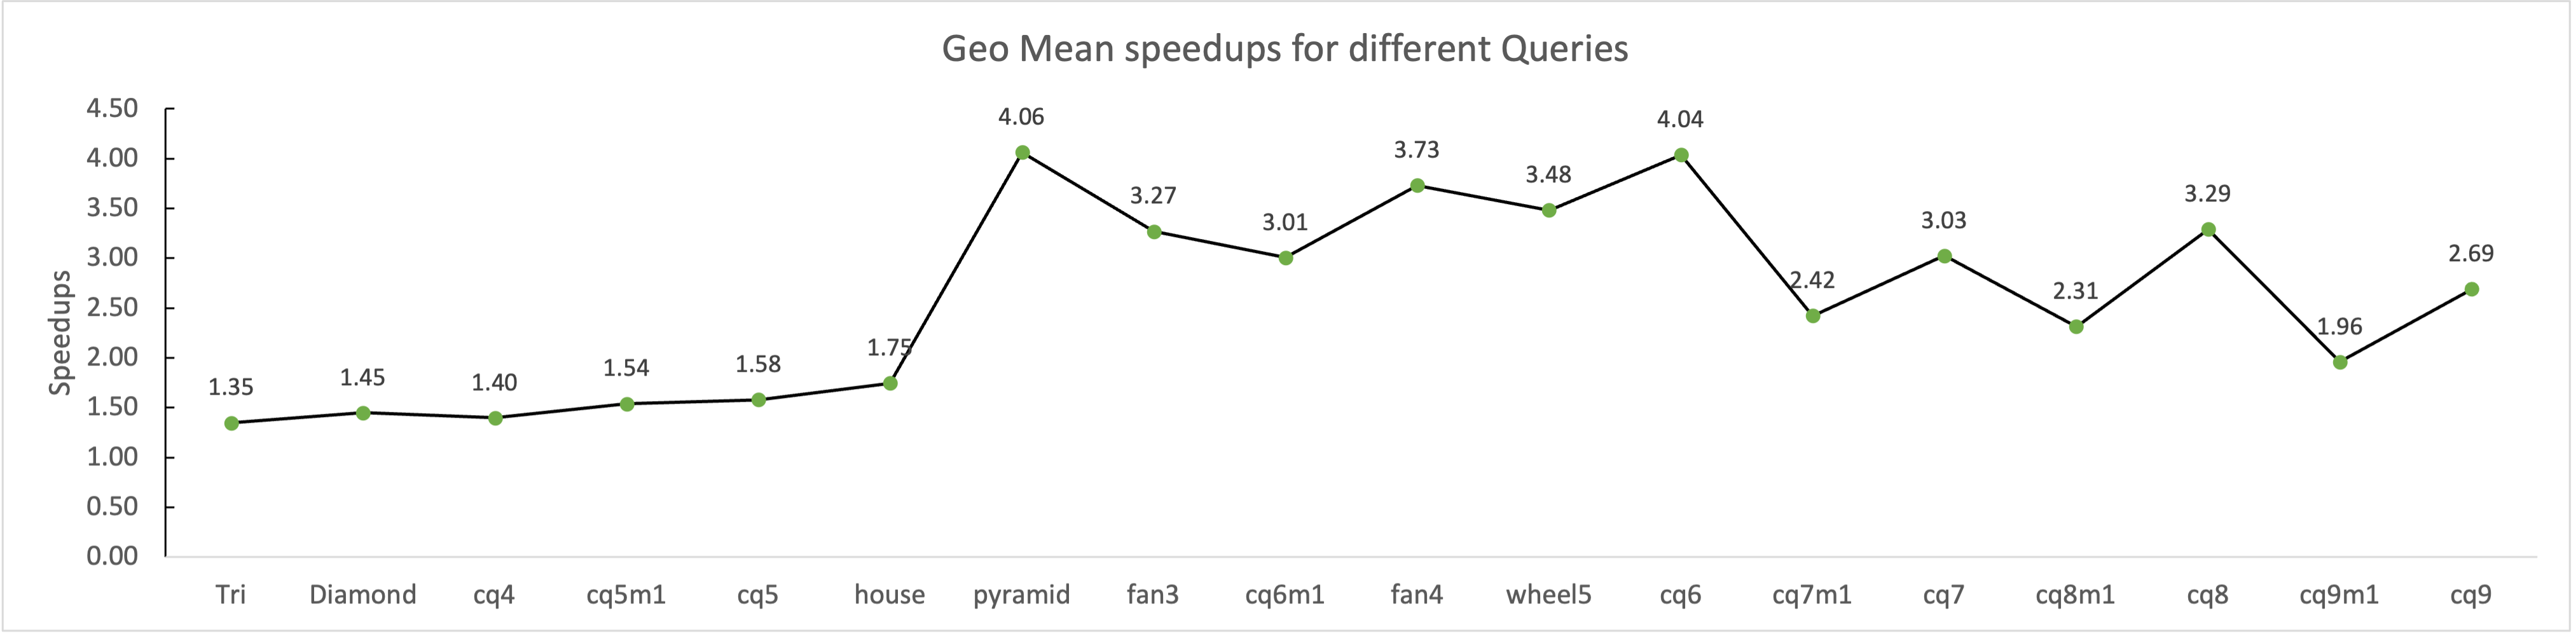
\includegraphics[width=\textwidth]{fig/Results/query-speedups.png}
    \caption{Geo Mean speedups across all data graphs}
    \label{fig:query-speedups}
\end{figure}
